% LaTeX Document for Android class @ THM
% \documentstyle[11pt]{article}
\documentclass[11pt,a4paper]{article}
\usepackage[ngerman]{babel}
\usepackage[utf8]{inputenc}
\usepackage{graphicx}
\usepackage{hyperref}
%\renewcommand{\ttdefault}{cmss}

\usepackage{lmodern}
\usepackage{amssymb}
\renewcommand{\familydefault}{\sfdefault}

%\newcommand{\changefont}[3]{
%\changefont{cmss}{m}{n} \changefont{cmss}{m}{sl} \changefont{cmss}{bx}{n} \selectfont}


% Default margins are too wide all the way around. I reset them here
\setlength{\topmargin}{-.5in}
\setlength{\textheight}{9in}
\setlength{\oddsidemargin}{.125in}
\setlength{\textwidth}{6.25in}
\begin{document}
\title{Memory - Dokumentation}
\author{A - Team\\Technische Hochschule Mittelhessen}
\renewcommand{\today}{26. Juli 2012}
\maketitle

\tableofcontents

\section {Prolog}
Die Gruppe A besteht aus Markus Kretsch, Frank Kevin Zey, Florian Thomas und Hagen Lauer.

\subsection{Anforderungen}

Muss
\begin{itemize}
\item Memory-Spielfeld mit sinnvoller Größe (z.B. 8x8 Karten/Felder) für 2 bis 6 Spieler.
\item Jeder Spieler bekommt einen Namen, der über Spielsitzungen hinweg gespeichert wird.
\item Über jeden Spieler wird eine Statistik angezeigt, wie z.B. Anzahl gewonnener \/ verlorener Spiele, oder Anzahl richtiger Treffer pro 100 Züge.
\end{itemize}
Kann
\begin{itemize}
\item Mehrspielermodus über mehrere Smartphones innerhalb eines LANs.
\item Weitere Spielkarten können z.B. von der SD-Karte nachinstalliert werden.
\end{itemize}
\subsection{Lösung / Idee}

\begin{itemize}

\item Bilder sollen mit Grid und Imageview dargestellt werden. Dabei bieten diese gute Möglichkeiten Klicks zu erkennen und entsprechend zu behandeln.
\item Für die Spieler wird eine SQLite Datenbank verwendet.
\item Wir haben gute Bibliotheken gefunden um die Daten der Spieler wie gewünscht statistisch auszuwerten und darzustellen.
\item Netzwerkspiele werden über WiFi und JavaSockets realisiert, dabei soll es einen Host und mehrere Clients pro Sitzung geben. Das Spielsystem muss also die entsprechende Flexibilität für lokale und Netzwerkspiele mitbringen.
\item Spielkarten sollen per .zip File von der SD Karte des Geräts nachladbar sein. Bilder werden in einer Datenbank gespeichert. Das Spiel lädt die Bilder für das Spielfeld aus der Datenbank.
\end{itemize}

\section{Installation}
Memory benutzt den \textbf{\href{https://github.com/JakeWharton/Android-ViewPagerIndicator}{ViewPagerIndicator}} von Jake Wharton. Um Memory kompilieren zu können muss deshalb es deshalb \href{https://github.com/JakeWharton/Android-ViewPagerIndicator/tarball/master}{heruntergeladen} werden.
\begin{itemize}
\item Gehen Sie nun in \textbf{Eclipse}, wählen File${\longrightarrow}$New${\longrightarrow}$Project${\longrightarrow}$Android Project from existing Code...${\longrightarrow}$ und wählen nun den \textbf{library} Ordner in dem eben heruntergeladenen ViewPagerIndicator-Verzeichnis aus.
\item Nachdem Sie die library Ihrem Workspace hinzugefügt haben, rechtsklicken Sie auf das Projekt und wählen Android Tools${\longrightarrow}$->Add Support Library aus und folgen den Instruktionen
\item Rechtsklicken Sie erneut auf das library-Projekt, wählen Properties${\longrightarrow}$Android aus und vergewissern sich, dass \textbf{is Library} ausgewählt ist. Gehen Sie nun in das Java Compiler-Menü und setzen das Java Compliance Level auf 1.6, da das Projekt nicht mit 1.7 zu laufen scheint.
\item Klicken Sie schließlich mit der rechten Maustaste auf das memory-Projekt, wählen Properties${\longrightarrow}$Android, klicken auf den \textbf{Add...} Button auf der rechten Seite und wählen das Library Projekt aus. Nun sollte das Projekt noch einmal bereinigt und neu kompiliert werden. Anschließend lässt dich die Applikation starten.
\end{itemize}
\section {Architektur}
Wir haben uns selbst als Ziel gesetzt, dass wir in 2 Richtungen entwickeln: Das Spiel Memory als sehr spezifische Implementierung und ein "'Framework"', das alle typischen Funktionen für ein rundenbasiertes Spiel mitbringt. So konnten wir mit entsprechenden Oberklassen (Game.java) und abgeleiteten Klassen (z.B. Memory.java) garantieren, dass am Ende beide Zweige zusammen führen.
Zum Framework gehört Game.java als Oberklasse aller implementierbaren rundenbasierten Spiele, eine Engine die im Wesentlichen Datenbankzugriffe kapselt, ein einfaches Menüsystem, das leicht konfigurier- und erweiterbar ist und einen statistischen Teil der mit der Datenbank zusammen arbeitet. Wir haben dann als Konkrete Implementierung für Memory die Klasse Memory.java von Game erben lassen und entsprechend für Memory angepasst. Ebenso wird die Netzwerkimplementierung eine von Game abgeleitete Klasse sein, natürlich noch mit einigen spezifischen Anpassungen zur Kommunikation der Geräte.\\\subsection{Design}
Wie in \autoref{fig:memorydesign} zu sehen ist entsteht das Framework völlig unabhängig vom zu implementierenden Spiel.
\begin{figure}[!h]
\centering
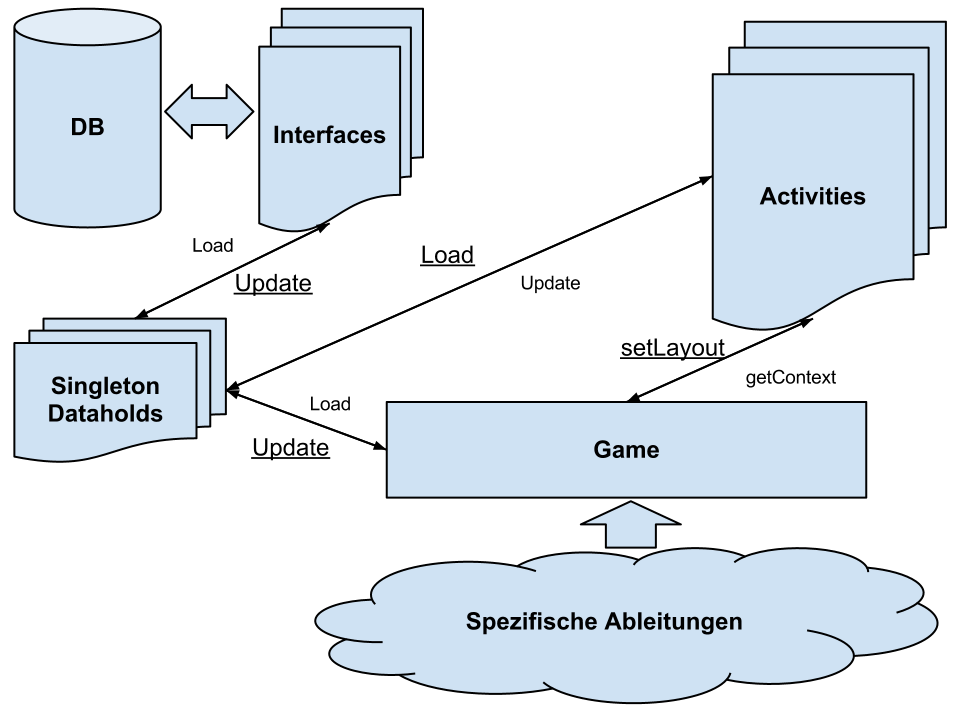
\includegraphics[scale=0.4]{pics/memorydesign.png}
\caption{Konzept}
\label{fig:memorydesign}
\end{figure}\\
Auf Grund einiger zeitlicher Probleme ist das Projekt dann doch etwas mehr ineinander Verwachsen als gedacht, jedoch hat der Grundgedanke der Unabhängigkeit dabei geholfen unser Projekt zu strukturieren und damit schnell zu implementieren. Gerade was die Datenbanken und das Spielinterface (die Menüführung) Angeht ist das Spiel durch die gezielte Verwendung von ListViews und die verschachtelten Menüs sehr leicht Anpassbar geworden und bietet in seiner grundsätzlichen Ausprägung auch genügend Funktionalität mit um einfache Spiele zu unterstützen. Die Memory-Erweiterungen beginnen im UI hauptsächlich bei den Settings: \autoref{fig:Activities}
\\
\begin{figure}[!h]
\centering
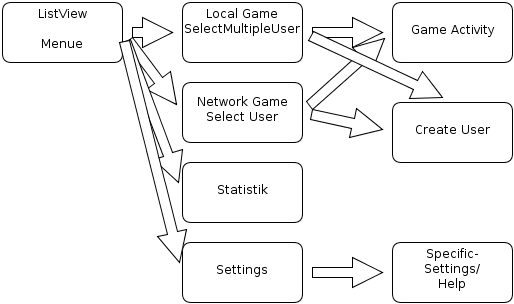
\includegraphics[scale=0.5]{pics/Activities.png}
\caption{Activity Diagramm}
\label{fig:Activities}
\end{figure}\\
In der Implementierung der Spieler-Typen macht die Frameworkausrichtung und die Benutzung von Oberklassen und Ableitungen etwas anschaulich: \autoref{fig:UMLPlayer}
\\
\begin{figure}[!h]
\centering
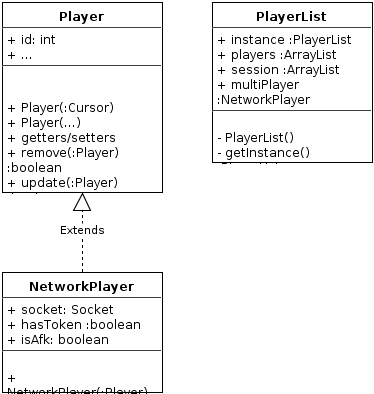
\includegraphics[scale=0.5]{pics/UMLPlayer.png}
\caption{UML Player Klassen}
\label{fig:UMLPlayer}
\end{figure}\\
Player ist hier eine Oberklasse, sie ist Teil des Frameworks. NetworkPlayer ist eine Ableitung, wobei hier noch nicht ganz klar ist ob sie Teil des Frameworks wird. Die Attribute könnten, sofern man denn einheitliche Netzwerkoperationen vorgibt, gut wiederverwendet werden. Die PlayerList ist ein reiner Datenlieferant der in der Regel beim Start der Applikation mit Daten befüllt wird. Das Objekt ist in der App einzigartig und wurde leider in der aktuellen Version etwas missbraucht für eher spezifische Eigenschaften der Memory-Implementierung. Dies wird allerdings im Code klarer und spielt hier keine große Rolle. Wichtig zu merken ist: Player werden in einem PlayerList Objekt gehalten. Dabei unterscheidet man noch in 2 Listen: Players, das sind alle aus der Datenbank gelesenen Spieler, und Session, das sind die zu einer Sitzung (lokales Spiel) gehörenden Spieler. Hintergrund war hier die Auftrennung für den Round Robin Algorithmus den wir beiderseits in Game.java als auch in Player.java realisiert haben. Dabei benötigt Game.java auch nur die Spielerliste der gerade teilnehmenden Spieler also nur Session. Die Spieler die in eine Session kommen werden in der SelectMultipleUserActivity ausgewählt.\\
Das Spiel und dessen Rundenprinzip ist in Game.java bzw. Memory.java realisiert. Essenziell ist dabei natürlich wie mit den Usereingaben umgegangen wird. In unserem Fall muss ein \emph{OnItemClickListener} implementiert werden. Wie, wann und wo dieser definiert und implementiert ist interessiert das Framework nicht. Es etwartet lediglich in der GameActivity, dass man dort an Stelle des traditionellen \emph{setContentView(int)} Aufrufs mit der Methode \emph{assemleLayout()} von Game.java ein View-Objekt erhält. Diese View ist dann Basis der Spielanzeige und ist frei konfigurierbar.
\\
\begin{figure}[!h]
\centering
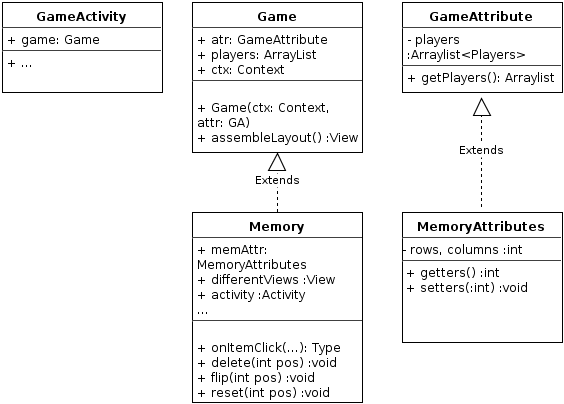
\includegraphics[scale=0.5]{pics/UML.png}
\caption{UML Game}
\label{fig:UML}
\end{figure}\\
Memory.java ereitert Game.java und überschreibt dabei z.B. die Methode \emph{assembleLayout()}. Die GameAttributes sind lediglich dazu gedacht mehr Flexibilität in die Architektur zu bringen, da unter Umständen dort für Initialisierungen etc. wesentlich mehr Attribute gebraucht werden könnten als wir sie bei Memory brauchen. Diese Attribute sollten, wenn man sie denn als Übergabe-Container verwendet in der gesamten Applikation zugreifbar gemacht werden. Im Falle von Memory werden die GameAttributes meistens an den Stellen erzeugt wo man sie auch tatsächlich benötigt. \\
Netzwerk und Kommunikation sollten in der GameActivity Klasse abgehandelt werden und bei bedarf über Methoden in die Game-Logik hereingereicht werden (z.B. Spielerwechsel mit \emph{turn()}). Die Netzwerk Implementierung ist auf Grund der knappen Zeit sehr spezifisch geworden, hier muss auf jeden Fall noch daran gearbeitet werden Protokolle zu erstellen auf deren Basis eine einheitliche Netzwerk-Implementierung mehrerer Spiele möglich ist. Das Thema Netzwerk wird noch genauer behandelt.

\subsection{Engine und Datenbank}
Die Engine umfasst die Typisierung der Spieler und Datenbankschnittstellen.
\subsubsection{Nachladen eines Kartendecks}
Beim Nachladen eines Kartendecks wird eine Zip File mit JPG Dateien erwartet. Diese Zip File muss eine JPG Datei mir Namen {\em 0.jpg} enthalten. Die Zip File wird aus der SD Karte geladen, dazu ist es zwingend notwendig, dass diese sich im root-Verzeichnis befindet.
Die Zip File wird von der Applikation geladen und entpackt. Während dem Entpacken werden die Informationen und einzelnen Bilder in einem deck Objekt gespeichert. Dabei kam es zu verschiedenen Problemen, einfachste Reader haben die jeweiligen Daten nicht aus dem Stream lesen können, somit wurde sich auf einen einfach InputStream geeinigt. Das ausgelesene Byte Array wurde anschliesend über eine BitmapFactory zu einem Bitmap Objekt dekodiert.\\
Wenn das Objekt vollständig erzeugt wurde, speichert es automatisch alle Daten in der Datenbank. Dabei kam es zu mehreren Problemen. Die Tabelle für ein Deck musste um eine weitere Tabelle in einer 1->n Beziehung ergänzt werden, nur so können alle Bilder mit Verweis auf das jeweilige Deck gespeichert werden.\\
Beim Laden der einzelnen Bilddaten kam es wegen den Streams wiedermal zu dem Problem, das ImageReader und ähnliche nicht wirkten, ein einfacher InputStream löst erneut das Problem.

\subsubsection{Allgemeines Datenbankdesign}
Die Datenbank umfasst 3 Tabellen. Diese Tabellen beinhalten die Informationen jedes einzelnen Spielers. Es wird der Nickname, die Siege, Niederlagen, sowie Unentschieden, getroffene Kartenpaare und die allgemein durchgeführten Züge gespeichert. Die jeweilige ID des Spielers entspricht dem jeweiligen Datensatz in der Datenbank.\\
Neben dem Spieler werden auch zusätzliche Kartendecks gespeichert. Da zu jedem Kartendeck es eine Rückseite vorhanden sein muss und 32 Vorderseiten, handelt es sich um eine 1 -$>$ n Beziehung. In der Datenbank werden zu jedem Kartendeck der Name gespeichert, dieser wird aus dem Dateinamen entnommen. Zusätzlich wird direkt die Rückseite in der Kartendeck Tabelle gespeichert, da die Rückseite nur einmal vorkommt und nicht noch aus der Kartentabelle gefiltert werden muss. Die Kartentabelle enthält die ID des jeweiligen Kartendecks als Referenz und einen Blob in dem die JPG Vorderseitenbilder als Byte Feld gespeichert wird.

Grösstes Problem während der Entwicklung des Datenbank Layouts waren immer wieder kleine Anpassungen durch ständige Weiterentwicklung der Software.

\subsection{Statistik}
Die Statistik wird mit Hilfe des Frameworks \textbf{\href{http://www.achartengine.org/}{Achartengine}} graphisch dargestellt. Dabei empfahl es sich für die Statistikanzeige der \"Treffer-Wahrscheinlichkeit\" ein Balkendiagramm mit jeweils zwei Balken pro Spieler zu verwenden. Um den Zahlenbereich der y-Achse passend zu wählen muss dafür der Spieler mit der höchsten Spielanzahl überhaupt aus der Datebank geholt werden und dieser Wert als Standardhöhe der y-Achse festgelegt werden.
Auch für die zweite Statistik, die \"Sieg-Wahrscheinlichkeit\" wurde ein Balkendiagramm der Achartengine verwendet, diesmal jedoch nur jeweils ein Balken. 
\subsubsection{Fragments}
Um den Wechsel zwischen den verschiedenen Statistiken ansprechender zu gestalten wurden statt Activities \textbf{Fragments} benutzt. Vereinfacht gesagt sind Fragments kleine Activities, die innerhalb einer Activity bestehen können und von der \textbf{\href{http://developer.android.com/tools/extras/support-library.html}{Support-Library}} bereitgestellt werden.
Um den Vorteil der Fragments noch besser herausstellen zu können wurde die externe Library \textbf{\href{http://viewpagerindicator.com/}{ViewPagerIndicator}} eingebunden. Mittels Paging  kann so durch die Statistiken navigiert werden, wie in \autoref{fig:stats} zu sehen ist.
\begin{figure}[!h]
\centering
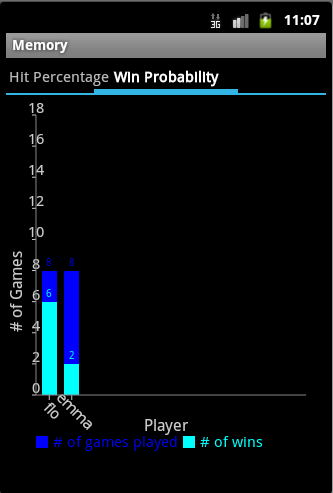
\includegraphics[scale=0.7]{pics/stats.png}
\caption{Statistiken}
\label{fig:stats}
\end{figure}
\subsection{Memory}
Aufrgund des Aufbaues eines Memoryspieles bietet es sich an ein GridView zu verwenden. Zur Visualisierung der verschiedenen Karten in dem GridView haben wir uns für die ImageViews entschieden, weil sie einfach zu verstehen sind. 
Die Bilder werden in der Klasse ``Theme`` aufbewart, welche diese aus der Datenbank liest, wenn es nicht das Default Theme ist. Dieses wird anhand von drawable Ressourcen geladen. Jedes Theme besteht aus einer Liste der Vorderseiten und einer Rückseite. \\
Das Memory lädt die ImageViews erstmal mit den Rückseiten in das GridView, weil man ja nicht sehen soll welche Karte sich darunter versteckt. Welches Bild sich wirklich unter dem Bild versteckt wird als id gespeichert. Wenn der User nun das erste Mal auf ein Bild klickt wird ein Zähler erhöht, um zu sehen ob das zweite Bilder gerade geklickt wird. Beim zweiten klick auf ein Bild  muss überprüft werden, ob es sich bei dem zweiten Bild

\begin{itemize}
	\item Um die selbe Position handelt 
	\item Ob sie die selbe id haben
\end{itemize}
	Für den Fall das die die selbe Position haben, wird der Zähler wieder runtergezählt, für den Fall, dass die ids identisch sind, werden die ImageViews disabled und das Bild auf null gesetzt, sodass der Anwender sieht, dass das Bild weg ist. Ansonsten werden die Bilder wieder zurückgesetzt. \\
Hier entstand das Problem, dass die Bilder sofort verschwanden und der User nicht sehen konnte was den unter der 2. Karte liegt. Aus diesem Grund haben wir Threads erstellt, die eine gewisse Zeit warten und dann erst gegebene Aktionen durchführen, wie zum Beispiel das Zurücksetzen oder das Löschen zweier Karten. \\
Dies führte dann aber zu dem Problem, dass der User klicken konnte während die Karten, die vorher angeklickt wurden, noch zu sehen waren und somit einige Eigenarten hervorhohlen konnten. Desswegen haben wir für diesen Zeitraum die ImageView disabled damit dies nicht passiert.\\
Unser Memoryspiel ist in der Lage auf viele zeilen/reihen 
Kombinationen zu reagieren. Aufgrund der Feldgröße 8x8 sollte ein 
Theme 32 Karten + Rückseite haben haben. \\
%Damit der Fall nicht auftritt, wo der User ein Theme importieren will mit weniger als 32 %Vorderseiten und der Rückseite, wird beim importieren überprüft, ob dies zutrifft, wenn nicht, %dann wird das Deck nicht importiert.
Um nun standartwerte benutzen/setzen zu können benutzen wir die Properties Klasse, welche einiges an Arbeit abnimmt. Die Konfigurationsdatei wird in dem lokalen Speicherbereich der Applikation gesichert. Um diesen herauszufinden benutzen wir die Funktion "getFilesDir()".\\
Diese wird beim Start ausgelesen, wenn nicht da oder unvollständig werden die Defaultwerte eingetragen, und bei den Settings gesetzt und auch geladen. \\
Beim laden des Memorys sind wir über den Fehler gestoßen, dass wir out of memory gegangen sind. Dies konnten wir beheben, indem wir in der Activity in der onDestroy methode die geladenen  Bitmaps wieder recyclen.

\subsection{Netzwerk}

\subsubsection{Server}
Wenn der Anwender der Applikation ein neues Netzwerkspiel startet, beginnt ein Service damit auf eingehende Verbindungen zu warten. Dieser Service (\textbf{HostService.java}) stellt den Server in einem Netzwerkspiel dar und übernimmt dafür typische Aufgaben wie das Verwalten der Client-Liste oder das Reagieren auf eingehende Nachrichten. Für jeden Client, der sich am Server anmeldet wird ein eigener Connection-Thread erstellt, der auf Nachrichten des entsprechenden Clients wartet (\textbf{ClientConnection.java}). Trifft eine Nachricht über die Socket-Verbindung ein wird ein neuer Thread einer Response-Klasse erstellt, welcher auf die eingegange Nachricht reagiert.
\subsubsection{Warteraum}
In der Warteraum-Activity befinden sich die Clients, nachdem sie sich mit dem Server verbunden haben. Der Server erkennt durch Überprüfung der Verbindungs-Sockets welcher Client auf dem selben Device wie der Host läuft. Dieser Host-Client hat auch als einziger die Möglichkeit das Spiel zu starten.
\subsubsection{Kommunikation}
Die Kommunikation zwischen den einzelnen Clients und dem Server wird über entsprechend kodierte Nachrichten realisiert. Bei bestimmten Ereignissen, z.B. dem Aufdecken einer Karte schickt der betroffene Client über seinen Outputstream eine Nachricht an den Server, die dieser über die oben beschriebenen Mechanismen aufnimmt, verarbeitet und an alle oder auch einzelne Clients weiterleitet.
Jeder Client wartet in einem AsyncTask auf eingehende Nachrichten. Ein Grund dafür ist, dass bei einem eingehenden Befehl so gut auf UI-Elemente zugegriffen werden kann. Wichtig ist, dass der AsyncTask der Warteraum-Activity beendet ist, wenn das Spiel im Gang ist, da nun eingehende Nachrichten keine ChatNachrichten sind, sondern Befehle, die im AsyncTask der GameActivity benötigt werden.
\subsubsection{Im Spiel}
Beim Laden des Spiels selbst wird die Spielfeldgröße zunächst auf die gewählte Spielfeldgröße des Hosts gesetzt. Anschließend wird auf dem Smartphone des Hosts die Verteilung der Karten berechnet und an alle Clients in einem String kodiert verschickt, so dass die Paarverteilung auf allen Smartphones gleich ist. Die Karten selbst können auf den teilnehmenden Smartphones unterschiedlich sein. Verlässt ein Spieler das Spiel vorzeitig durch Betätigen des "Zurück-Buttons" wird das Spiel bei allen Spielern beendet. Wird ein Spiel ordnungsgemäß beendet verschickt der Spieler, der mit seinem Zug die letzten Karten entfernt hatte, an alle Spieler eine Nachricht über die Beendigung des Spiels, so dass diese auch die GameActivity beenden, einen möglichen Sieger einblenden und anschließend wieder zur WaitingRoomActivity zurückkehren.
Nun kann auch der Chat wieder benutzt werden, weitere Spieler können hinzukommen und der Hostspieler kann jederzeit eine neue Runde starten.
\subsection*{Benutzerdokumentation}

Die Benutzerdokumentation wird per {\em Help} in der App bereitgestellt. 

\subsection*{API Dokumentation}

Die Code Dokumentation ist per JavaDoc im Quelltext abgewickelt.

\subsection*{Repository}

http://github.com/Crunch09/memory \\
git://github.com/Crunch09/memory.git

\end{document}
